\documentclass[14pt]{beamer}

%%%%%%%%%%%%%%%%%%%%%%%%%%%%%%%%%%%%%%%%%%%%%%%%%%%%%%%%%%%
%%%%%%%%%%%%%%%%%%%%%%%%%%%%%%%%%%%%%%%%%%%%%%%%%%%%%%%%%%%


\usepackage[orientation=portrait]{beamerposter}
	\usepackage{amsmath, amssymb}
	\usepackage{microtype}
	\usepackage{empheq}
	\usepackage{siunitx}
	\usepackage{dsfont}

	\usepackage{tikz}
	\usetikzlibrary{patterns,arrows,decorations.pathreplacing,hobby}
	\usepackage{graphicx}
\usepackage{natbib}
\usepackage{fontspec}
\setsansfont{Palatino}

\usetheme{Berlin}      % or try Darmstadt, Madrid, Warsaw, ...
\usecolortheme{rose} % or try albatross, beaver, crane, ...
%\usefonttheme{serif}  % or try serif, structurebold, ...
\setbeamertemplate{navigation symbols}{}
\setbeamertemplate{caption}[numbered]

	\newcommand{\cit}{\textbf{[$\blacksquare$] }}

\renewcommand{\maketitle}{%
	\begin{center}%
		\Huge\inserttitle\\[5mm]%
		\Large\insertauthor\\[5mm]%
		\Large\insertinstitute%
	\end{center}%
	\vspace*{-1.5ex}%
}

\geometry{
  hmargin=2.5cm, % little modification of margins
}

\setlength{\paperwidth}{24in}
\setlength{\paperheight}{36in}
\setlength{\textwidth}{\paperwidth}
\setlength{\textheight}{0.9\paperheight}
\setbeamersize{text margin left=0.5cm,text margin right=0.5cm}

% beamer definitions

\makeatletter
\definecolor{lightblue}{RGB}{33,140,168}
\definecolor{crimson}{RGB}{218,61,73}
\definecolor{cream}{RGB}{250, 245, 245}
\definecolor{clay}{RGB}{207, 190, 180}

\setbeamercolor{normal text}{fg=black,bg=white}

\setbeamercolor{block body}{fg=black, bg=lightblue!20!white}
\setbeamercolor{block title}{fg=white, bg=lightblue!60!black}


\setbeamercolor{alerted text}{fg=crimson}


\setbeamercolor{example text}{fg=crimson!50!black}
\setbeamercolor{block body example}{fg=black, bg=cream!80!gray} 
\setbeamercolor{block title example}{fg=white, bg=crimson} 

\setbeamercolor{structure}{fg=cream}

\setbeamercolor{background canvas}{bg=cream, parent=normal text}
\setbeamercolor{background}{parent=background canvas}

\setbeamercolor{palette primary}{fg=cream!40!white,bg=crimson!80!black}
% \setbeamercolor{palette secondary}{use=structure,fg=structure.fg!100!green}
% \setbeamercolor{palette tertiary}{use=structure,fg=structure.fg!100!green} 

\makeatother

%%%%%%%%%%%%%%%%%%%%%%%%%%%%%%%%%%%%%%%%%%%%%%%%%%%%%%%%%%%
%%%%%%%%%%%%%%%%%%%%%%%%%%%%%%%%%%%%%%%%%%%%%%%%%%%%%%%%%%%

\title{Characterizing Computational Techniques for Experimentally Feasible Non-Local Evolution of Two-Qubit Systems}
\author{Shankar Balasubramanian\hspace{1em} Didi Chang-Park\hspace{1em} Kyle Herndon\hspace{1em} Zane Rossi}
\institute{TJHSST Modern Physics and Optics Lab}
\date{9 June 2015}

\begin{document}
\centering
	\begin{frame}{\maketitle}
	
		%		\begin{block}{Abstract}
					   {\bf{Abstract:}} This paper investigates computational methods and presents a computational framework for simulating non-local evolution of two-qubit systems. This evolution may then easily be combined with finite local operations to give control of near-arbitrary precision. Current research has focused on developing the theoretical background which we hope to computationally implement. We will characterize how useful operators (particularly the $CNOT$ gate) are generated in this process, and they will be approximated and performed computationally in optimal time utilizing a adaptive-algorithm approach. We will also analyze the non-local piece of the system Hamiltonian, including determining experimental means of generating it.  Particularly, we will be evaluating its action on the Poincar\'{e}-Bloch-Sphere.
%\end{block}
\vfill

		\begin{columns}
			\begin{column}{.45\textwidth}
			
\begin{exampleblock}{Mutation Protocol}

		\begin{figure}[htpb]
		\centering
			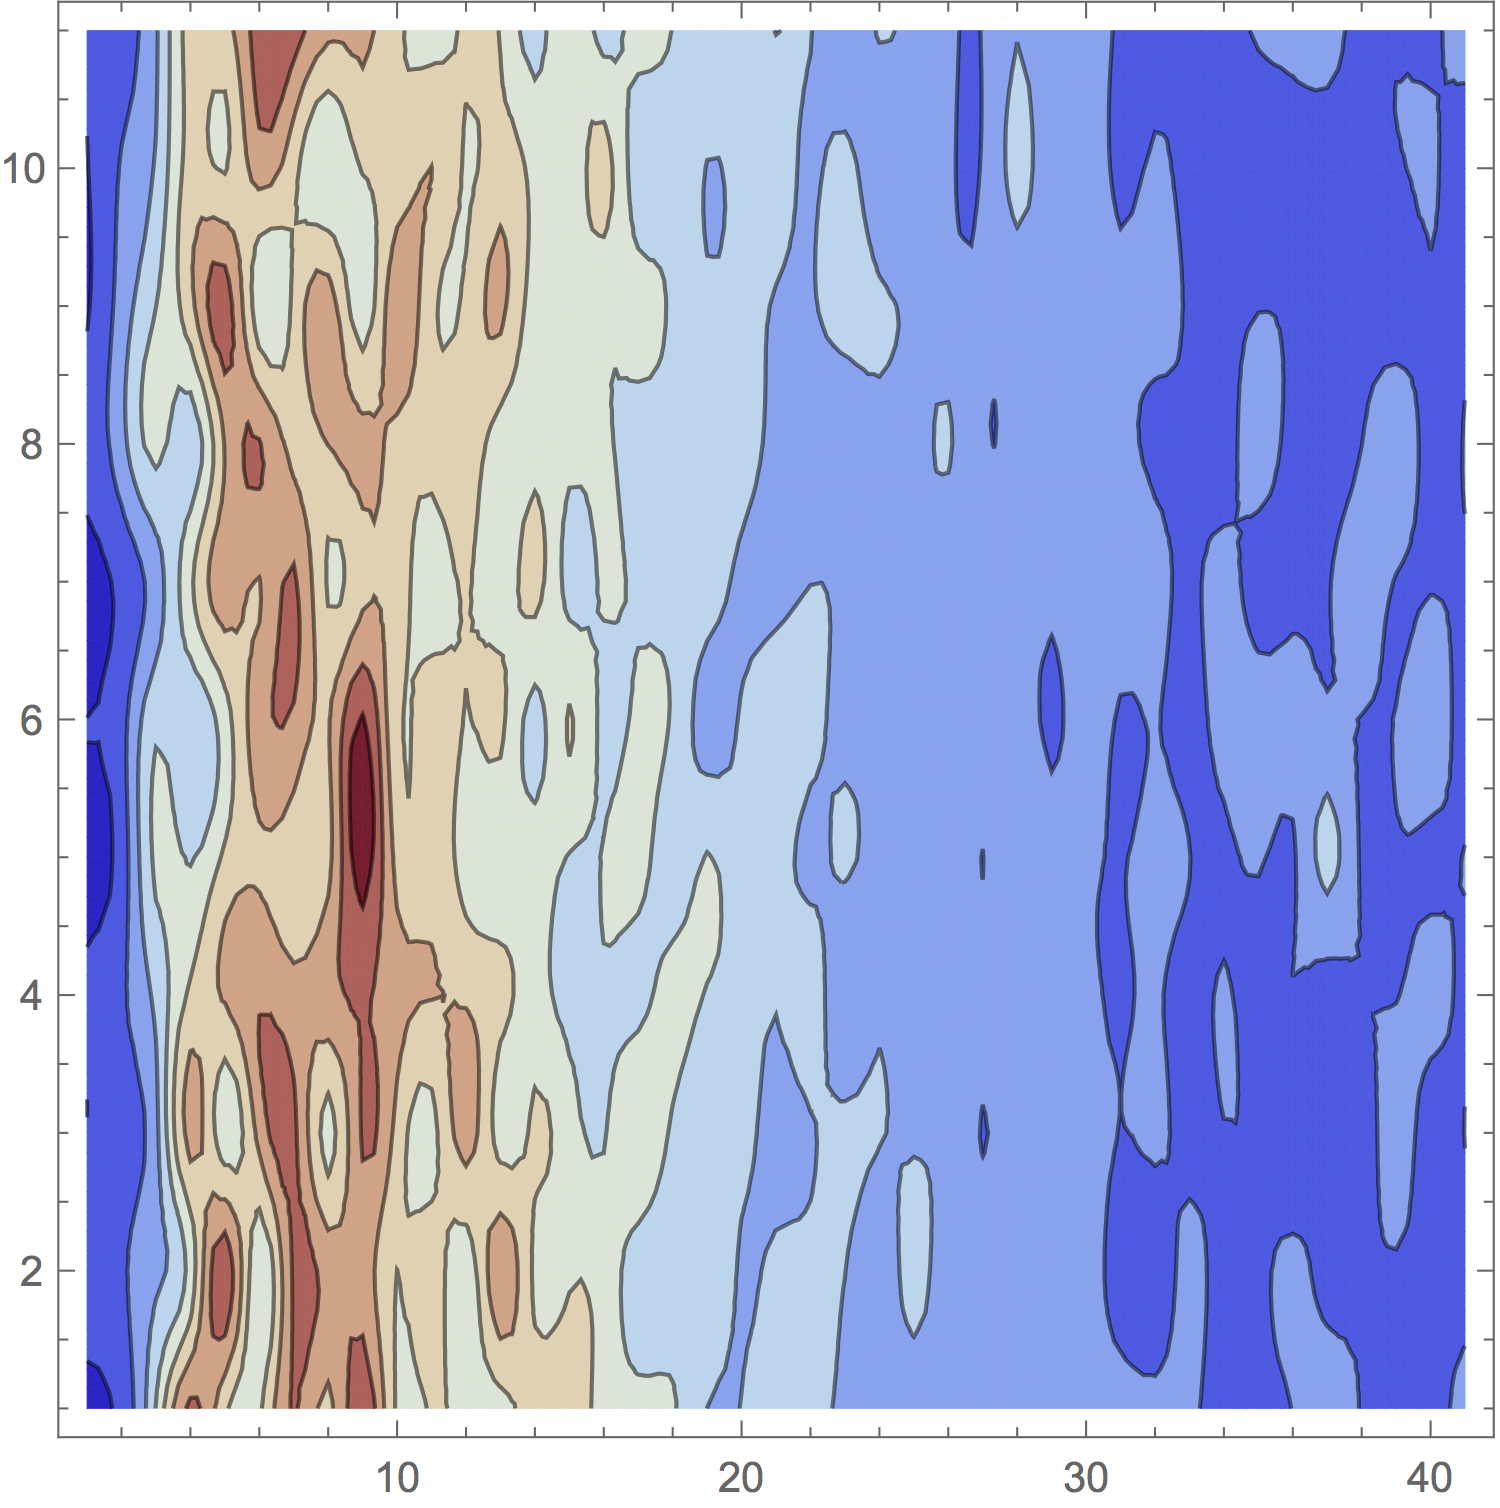
\includegraphics[scale=1.3]{cp1.png}
		\centering
		\caption{This plot shows the fidelity of the best organism in a ten-organism set after $100$ generations with respect to mutation chance and mutation magnitude. The vertical axis, when the value is multiplied by $0.1$, gives the chance in any generation for one of the angles defining an organism to be mutated. The horizontal axis, when multiplied by $0.025$, gives the mutation magnitude (this ranges between $0$ and $1$ radian(s)). The plot shows clear correlation between mutation magnitude and organism success.}
		\label{fig:effplot}
	\end{figure}

	Mutations are designated on the basis of chance and magnitude. We set a particular threshold value, which we are free to change. This threshold value ($\alpha$) determines whether or not a particular organism's parameters will be mutated. The parameters, as discussed above, are the $\beta '$ rotation coefficients which are specified in the exponential form of the local operations. The other changeable parameter, $\mu$, specifies the degree to which the angles will be mutated. These mutations encompass an envelope of random values between $-\mu$ and $\mu$  (a uniform distribution) which will be added to the current $\beta'$ values to update them.  Figure \ref{fig:effplot} depicts the efficacy of the simulation (particularly, the fidelity), for different values of $\alpha$ and $\mu$.  Lighter colors represent simulations resulting in higher fidelities. The values of $\alpha$ and $\mu$ do not change across the entire simulation; however, the efficiency of our program can be increased by modifying these values per each generation

\end{exampleblock}
\vspace{1em}

\begin{block}{The Space as a Whole}

	\begin{figure}[htpb]
		\centering
			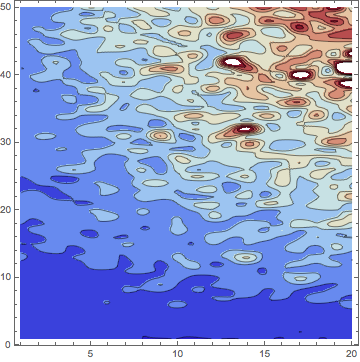
\includegraphics[scale=1.3]{cp2.png}
		\centering
		\caption{Caption. Caption. Caption. Caption. Caption. Caption. Caption. Caption. Caption. Caption. Caption. Caption. Caption. Caption. Caption. Caption. Caption. Caption. Caption. Caption. Caption. Caption. Caption. Caption. Caption Caption. Caption. Caption. Caption. Caption. Caption. Caption. Caption. Caption. Caption. Caption. Caption. Caption.. Caption.  Caption. Caption. Caption. Caption. Caption. Caption. Caption. Caption. Caption. Caption. Caption. Ca Ca Caption. Caption. Caption. Caption. Caption. Caption. Caption. Caption. Caption. Caption. Caption. Caption. Caption. Caption. Caption. Caption. Caption. Caption. Caption. Caption. Caption. Caption. Caption. Caption. Caption. Caption.ption. Caption. Caption. Caption. Caption. Caption. Caption. Caption. Caption. Caption. Caption. Caption. Caption.ption. Caption. Caption. Caption. Caption. Caption. Caption. Caption. Caption. Caption. Caption. Caption. Caption. Caption. Caption.Caption. Caption. Caption. Caption. Caption. Caption. Caption.}
		\label{fig:tot_plot}
	\end{figure}
	
\end{block}
\vspace{1em}
\begin{exampleblock}{Fig}
	\begin{figure}[htpb]
		\centering
			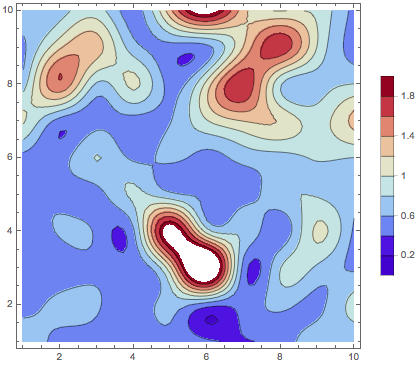
\includegraphics[scale=1.3]{thing.png}
		\centering
		\caption{ Caption. Caption. Caption. Caption. Caption. Caption. Caption. Caption. Caption. Caption. Caption. Caption. Caption. Caption. Caption. Caption. Caption. Caption. Caption. Caption. Caption. Caption. Caption. Caption. Caption Caption. Caption. Caption. Caption. Caption. Caption. Caption. Caption. Caption. Caption. Caption. Caption. Ca Caption. Caption. Caption. Caption. Caption. Caption. Caption. Caption. Caption. Caption. Cap Caption. Caption. Caption. Caption. Caption. Caption. Caption. Caption. Caption. Caption. Caption. Caption. Caption. Caption. Caption. Caption. Caption. Caption. Caption. Caption. Caption. Caption. Caption. Caption.tion. Caption. Caption. Caption. Caption. Caption. Caption. Caption. Caption. Caption.ption.. Caption. Caption. Caption. Caption. Caption. Caption. Caption. Caption. Caption. Caption. Caption. Caption. Caption. Caption. Caption. Caption. Caption. Caption. Caption. Caption. Caption. Caption. Caption. Caption.}
		\label{fig:thing_plot}
	\end{figure}
\end{exampleblock}


%%%%%%%%%%%%%%%%%%%%%%%%%%%%
\end{column}
%%%%%%%%%%%%%%%%%%%%%%%%%%%
							
			\begin{column}{.45\textwidth}
			\begin{block}{Variation in Population}

	A series of methods is used to determine fidelity in a populations of a set size, generation number, and gene length. We can then produce a series of partially-evaluated functions that can be mapped over a list of integers. When the results of this mapping are plotted, we gain knowledge of a slice of the search space. Knowledge of these slices, analogous to partial derivatives, can help determine which variables produce the best solutions with the smallest computational cost. 

	\begin{figure}[htpb]
		\centering
			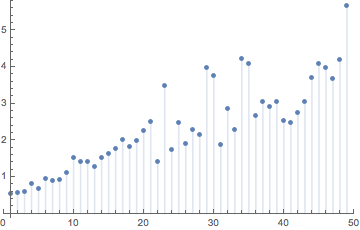
\includegraphics[scale=1.3]{g1.png}
		\centering
		\caption{A plot of the average of $20$ runs in which the population is along the horizontal axis, and fidelity ($\mathcal{F}$), is along the vertical axis. During these runs, the organism population was brought through $20$ generations, with each organism having two genes. The mutation chance ($\alpha$) and mutation magnitude ($\mu$) are drawn from the maximum of Figure \ref{fig:effplot} ($0.5$ and $0.225$ respectively).}
		\label{fig:pop_plot}
	\end{figure}

	Here we see a plot of constant generation number and gene length, where population size is being altered. Over a large average, the upward trend is clearly visible, as would make sense, and closely follows an exponential trend. We can conjecture that, given a saturation of the space with organism, we may eventually approach a point of diminishing returns, but that is not apparent in Figure \ref{fig:pop_plot}. These factors indicate a volatile variable, where we are sacrificing memory for some time and search space-covering. 
\end{block}
\vspace{1em}
\begin{exampleblock}{Variation in Generation Number}

	The same process is used as described above, save now the slice through the search space is made in a way orthogonal to the original slice. On average, due to the structure of the space, the behavior along one slice is related to that at adjacent slices. We see a similar but not identical behavior. 

	\begin{figure}[htpb]
		\centering
			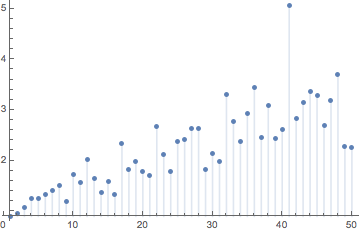
\includegraphics[scale=1.3]{g2.png}
		\centering
		\caption{A plot of the average of $20$ runs in which the generation number is along the horizontal axis, and fidelity is along the vertical. During this run, the number of generations is taken from $1$ to $50$, while the gene number remains at $2$, and the population is constant at $20$. ($\alpha$ and $\mu$ are preserved from Figure \ref{fig:pop_plot})}
		\label{fig:gen_plot}
	\end{figure}

	There is still a general upward trend when the data are aggregated. However, the growth with respect to generation number appears more logarithmic in character. This view is highlighted further in the paths along Figure \ref{fig:tot_plot}. These factors indicate that generation number is not as volatile a variable. 

	There are a number of explanations for this, but the most intuitive is that that size of the space is simply too large to be worked through by mutation alone. When there are few organisms, they stay within a close neighborhood of their original location (when breeding is not introduced, as it was not in these plots.) However, when the initial system is widely populated, each organism can work with the others to `patch' the space. 
\end{exampleblock}				\vspace{1em}

\begin{block}{Random shit}
\begin{figure}[htpb]
		\centering
			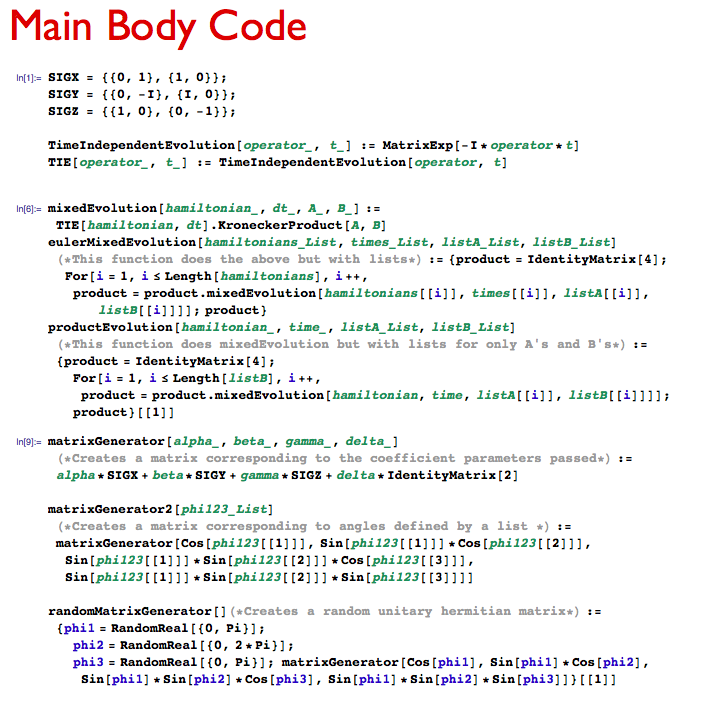
\includegraphics[scale=1.1]{code.png}
		\centering
		\caption{A plot of anarchy.}
		\label{fig:anarch_plot}
	\end{figure}


\end{block}
							\end{column}
	
		\end{columns}
	\end{frame}

%%%%%%%%%%%%%%%%%%%%%%%%%%%%%%%%%%%
%% Half slides %%%%%%%%%%%%%%%%%%%%%%%%%%%	
	\begin{frame}
		\begin{columns}
			\begin{column}{.45\textwidth}
				\begin{exampleblock}{Background}
					The ultimate goal of Control Theory is the ability to arbitrarily manipulate the state of an ensemble of qubits. In the context of quantum computation, this problem is reduced further: basic quantum gates allow for modular systems \cite{bremner}. However, the generation of these gates is non-trivial, and the arbitrary Hamiltonian is, in general, not readily constructible. Often one will wish to achieve a specific unitary evolution operator or gate $U$ corresponding to the solitary time evolution of a Hamiltonian $H$. When $H$ may not be engineered easily, the evolution can be achieved in other ways \cite{bremner} , often involving the use of local operations (LO), repeated measurements on the system \cite{bennett}, along with standard Hamiltonian-driven evolution drawing from some collection (possibly a one element collection) $H_1, H_2, \cdots, H_n$, all of which \emph{can} be lucratively generated.

	In the simplest case, a two particle system, the Hamiltonians involved may contain non-local terms, usually corresponding to particle-particle interactions. This paper will propose a framework for taking the general non-local Hamiltonian \cite{bennett} 
	\begin{equation}
	H = A \otimes \mathds{1} + \mathds{1} \otimes B + \sum_{ij} M_{ij}\,  \sigma_i \otimes \sigma_j
	\end{equation}
	and interspersing its non-local part's evolution with LO to achieve a desired $U$. It is only the non-local part of the Hamiltonian which must be studied, and through decomposition of this piece into its canonical form, and some insight into Lie Theory, we are able to formulate a computational approach \cite{haselgrove}. Devising a scheme to generate a $U$ from a collection of available operators and Hamiltonians has direct applicablity to a variety of problems, but cannot be done purely analytically on a massive scale, thus making a computational method necessary.
				\end{exampleblock}
				\begin{block}{Adaptive Algorithm Theory}
	Adaptive algorithms attempt to mimic the process of evolution by the mechanisms of mutation and natural selection. A set of mathematical objects dubbed \emph{organisms}, each containing some set of data, are subjected to tests against some metric depending on the organism's features \cit. This is considered one \emph{generation}, and the best organisms of each generation are bred together (by some deterministic algorithm) and mutated to compete in the next generation.

	In preparation for performing a process like the one described, we take three major steps.
	\begin{itemize}
	\item To begin, the degrees of freedom of the system should be analyzed, as these will function as the dimensions of the search space. During this process, the degrees which are less pertinent to a solution's fidelity should be identified and their relative mutation amplitude and frequency altered accordingly.

	\item Next, the mutations assigned to each degree of freedom will be designed so as to best approach a (hopefully) global extrema in the search space. In general, more volatile mutations will be given to the more effective degrees of freedom, and all mutations will decrease in magnitude and frequency as the number of generations increases \cit. 

	\item Finally, we need determine the method by which the best organisms of each generation are bred (combined in a way that may retain traits of both.). Note that there is no guarantee under any binary operation that the resulting object will have the same advantages assigned to the parent objects. In the case of well-defined and relatively smooth systems, this breeding will often resemble a sort of average, and the child will often perform similarly to the parents. 
	\end{itemize}
	With these in mind, we can visualize the process as a sort of traversal of a complex multidimensional search space. This will give some heuristic for the arguments for convergence.
\begin{figure}[htpb]
	\centering
	\begin{tikzpicture}[scale=1.5, use Hobby shortcut]

	% main bounding shape
	\draw[ultra thick, closed=true, dash pattern=on 6pt off 6pt] (2.5,4.5) .. (3.3,6.5) .. (5,7.5).. (7.5,7.9).. (10,7.5).. (11,6.5).. (11,4.5) ..(8.5,2).. (6,3.5).. (3,2).. (2.5,4.5);

	%interior grid
	\begin{scope}
		\clip[closed=true] (2.5,4.5) .. (3.3,6.5) .. (5,7.5).. (7.5,7.9).. (10,7.5).. (11,6.5).. (11,4.5) ..(8.5,2).. (6,3.5).. (3,2).. (2.5,4.5);

		\draw[step=1,gray,thick] (0,0) grid (15,15);
	\end{scope}

	% organism paths
	\draw[ultra thick, color=lightblue] (4.5, 4.5) -- (6.5, 4.5);
	\draw[ultra thick, color=crimson, dash pattern=on 0.2cm off 0.2cm] (4.5, 4.5) -- (6.5, 4.5);
	% yeah, that's right, I just did that (dashed overlay)
	\draw[ultra thick, -latex, color=lightblue] (6.5, 4.5) -- (7.5,4.5) -- (7.5,3.5) -- (8.5,3.5) -- (8.5,7.5);
	\draw[ultra thick, -latex, color=crimson] (6.5, 4.5) -- (6.5,6.5);

	% organism circle
	\fill[fill=lightblue] (4.5,4.5) circle (0.4cm);

	% organism symbol and arguments
	\node[right] at (-0.5, 9) {\large{$\Theta:\;$ \small{\sc{Arguments}}}};
	\draw (-0.5, 8.5) -- (4, 8.5);

	\node[right] at (-0.5, 6) {$\{A_i\}\;\;\{B_i\}$};
	\node[right] at (-0.5, 5) {$\{t_i\}\;\;$};
	\node[right] at (-0.5, 8) {$H:\;$ \small{\sc{Constant}}};
	\node[right] at (-0.5, 7) {$N:\;$ \small{\sc{Constant}}};

	\end{tikzpicture}
	\centering
		\caption{
		This is a simplification; the organism being tested is represented by the circle in blue, while the search-space (which has a defined metric represented by the grid) surround it. The paths of different color shown represent the non-deterministic paths possible as the organism mutates and is bred with other successful organisms. The actual space being searched is not two- but many-dimensional.
		}
	\end{figure} 
\end{block}
				\vspace{1em}
	\begin{exampleblock}{Geometry of the 3-Sphere}

\end{exampleblock}

%%%%%%%%%%%%%%%%%%%%___ COMPUTE ___%%%%%%%%%%%%%%%%
%%%%%%%%%%%%%%%%%%%%%%%%%%%%%%%%%%%%%%%%%%%%%%%%%%%

					\end{column}
			
			\begin{column}{.45\textwidth}
			
				\begin{block}{Arguments \& Degrees of Freedom in the Test Organism}
	%%%%%%%%%%%%%%%%%%%%%%%%%%%%%%%%%%%%%%%%%%%%%%%%%%%%%%%


	For the adaptive algorithm process described, each organism, denoted $\Theta$, is given a set of arguments which define it and serve as its characteristics. For our purposes, these can be further divided into \emph{constants} and \emph{mutables}. 

	Among the constants, we have $H$, a set Hamiltonian that is easy to generate, and is used in every free evolution between LO. It does not change in each simulation, across all organisms, and across all generations. We also have $N$, which defines the number of LO-FE pairs for all organisms in a given simulation. None of these variables is subject to the mutation protocol that defines adaptive algorithms. 

	\begin{equation}
		\underbrace{  (A_1\otimes B_1)e^{-i H t_1}\cdots(A_{N}\otimes B_{N})e^{-i H t_{N}}}_{N}
	\end{equation}

	The mutable data contains all of the sets. This includes the set of $A_i$, which are unitary operators on the first particle, the set of $B_i$, which are unitary operators on the second particle, and the set of $t_i$, which are the discrete durations for each FE, and have the constraint of summing to a particular value.
	
	In any effective adaptive algorithm, the structure of the search space must be known. This allows both a functioning and efficient algorithm. In this scenario, the dimension of the space depends on the step number $N$ in a linear fashion. We begin with a local operation, $A$, which is of the form

	\begin{equation}
		\beta \cdot \sigma 
		= 
		\begin{pmatrix}
			\beta_0 + \beta_3    &    \beta_1 - i \beta_2\\[3mm]
			\beta_1 + i \beta_2  &    \beta_0 - \beta_3
		\end{pmatrix}
	\end{equation}

	This appears to have four degrees of freedom, one for each element of $\beta$. However, there is an implicit restraint given the unitarity of the LO, we may recognize this as an exponentiation of a linear combination of the pauli-matrices. 

	\begin{equation}
		A^{\dagger}A = \mathds{1} \implies A = \mathds{1}\cos{|\beta'|} + (\beta' \cdot \sigma) \sin{|\beta'|}
	\end{equation}

	And we recognize this form as being equivalent to the specification of a single point by a new vector $\beta'$ on the three sphere. Thus $A$ is also equivalent to 

	\begin{equation}
		exp\{\beta' \cdot \sigma\} = exp\{\beta'_1 \sigma_1 + \beta'_2 \sigma_2 + \beta'_3 \sigma_3 \}
	\end{equation}

	This gives six degrees of freedom for each pair of local operations. We also note that given variability in the discrete FE times, we would be given $N-1$ more degrees of freedom (the restriction is due to their sum being defined). All considered,  we are searching a $6N$-dimensional space for every $N$-family.



				\end{block}

				\begin{exampleblock}{Conclusion}
					
					
				\end{exampleblock}
				\vspace{1em}
				
				\begin{block}{References}
					\bibliographystyle{plain}
				\bibliography{ref}		
				\end{block}
			\end{column}	
		\end{columns}
	\end{frame}	
\centering


\end{document}